\let\negmedspace\undefined
\let\negthickspace\undefined
\documentclass[journal]{IEEEtran}
\usepackage[a4paper, margin=10mm, onecolumn]{geometry}
\usepackage{lmodern} % Ensure lmodern is loaded for pdflatex
\usepackage{tfrupee} % Include tfrupee package

\setlength{\headheight}{1cm} % Set the height of the header box
\setlength{\headsep}{0mm}  % Set the distance between the header box and the top of the text

\usepackage{gvv-book}
\usepackage{gvv}
\usepackage{cite}
\usepackage{amsmath,amssymb,amsfonts,amsthm}
\usepackage{algorithmic}
\usepackage{graphicx}
\usepackage{float}
\usepackage{textcomp}
\usepackage{xcolor}
\usepackage{txfonts}
\usepackage{listings}
\usepackage{enumitem}
\usepackage{mathtools}
\usepackage{gensymb}
\usepackage{comment}
\usepackage[breaklinks=true]{hyperref}
\usepackage{tkz-euclide} 
\usepackage{listings}
% \usepackage{gvv}                                        
\def\inputGnumericTable{}                                 
\usepackage[latin1]{inputenc}                                
\usepackage{color}                                            
\usepackage{array}                                            
\usepackage{longtable}                                       
\usepackage{calc}                                             
\usepackage{multirow}                                         
\usepackage{hhline}                                           
\usepackage{ifthen}                                           
\usepackage{lscape}
\usepackage{tikz}
\usetikzlibrary{patterns}

\begin{document}

\bibliographystyle{IEEEtran}
\vspace{3cm}

\title{1.1.6.14}
\author{EE25BTECH11064 - Yojit Manral}

\maketitle
% \maketitle
% \newpage
% \bigskip
{\let\newpage\relax\maketitle}
\renewcommand{\thefigure}{\theenumi}
\renewcommand{\thetable}{\theenumi}
\setlength{\intextsep}{10pt} % Space between text and float

\textbf{Question:}\\
Find the vector equation of the plane passing through the points $\vec{R}\brak{2, 5, -3}$, $\vec{S}\brak{-2, -3, 5}$ and $\vec{T}\brak{5, 3, -3}$.\\

\textbf{Solution:}\\
\begin{table}[h!]    
  \centering
  \begin{tabular}[12pt]{ |c| c|}
    \hline
    \textbf{Points} & \textbf{Name}\\ 
    \hline
	\myvec{7\\10} & Point $\Vec{A}$ \\
    \hline 
	\myvec{-2\\5} & Point $\Vec{B}$\\
    \hline
	\myvec{3\\4} & Point $\Vec{C}$\\
    \hline
\end{tabular}
  \caption{List of Points}
  \label{Table_1}
\end{table}\\

$\rightarrow$ We can write the equation for the required plane as
\begin{align} \vec{n}^{T}\vec{x} = c \end{align}
$\rightarrow$ Also, $\vec{R}$, $\vec{S}$ and $\vec{T}$ satisfy this equation. Hence
\begin{align}
    \vec{n}^{T}\vec{R} = c \\
    \vec{n}^{T}\vec{S} = c \\
    \vec{n}^{T}\vec{T} = c
\end{align}
$\rightarrow$ From (1), (2), (3) and (4), we get
\begin{align} \vec{n}^{T}\myvec{\vec{R} & \vec{S} & \vec{T}} &= c\myvec{1 & 1 & 1} \end{align}
$\rightarrow$ Using transpose on both sides, we get
\begin{align}
    \myvec{\vec{R} & \vec{S} & \vec{T}}^{T} \vec{n} &= c\myvec{1\\1\\1} \\
    \vec{n} &= c \brak{\myvec{\vec{R} & \vec{S} & \vec{T}}^{T}}^{-1} \myvec{1\\1\\1} \\
    &= c \brak{\myvec{2 & -2 & 5 \\ 5 & -3 & 3 \\ -3 & 5 & -3}^{T}}^{-1} \myvec{1\\1\\1} \\
    &= c \myvec{2 & 5 & -3 \\ -2 & -3 & 5 \\ 5 & 3 & -3}^{-1} \myvec{1\\1\\1} \\
    &= \frac{c}{56} \myvec{-6 & 6 & 16 \\ 19 & 9 & -4 \\ 9 & 19 & 4} \myvec{1\\1\\1} \\
    &= \frac{c}{7} \myvec{2\\3\\4}
\end{align}
$\rightarrow$ From (11), we get the value of
\begin{align} \vec{n} = \myvec{2 \\ 3 \\ 4} \end{align}
$\rightarrow$ From (2) and (12), we get
\begin{align} c = \myvec{2 & 3 & 4} \myvec{2 \\ 5 \\ -3} = 7 \end{align}

\begin{figure}[h!]
   \centering
   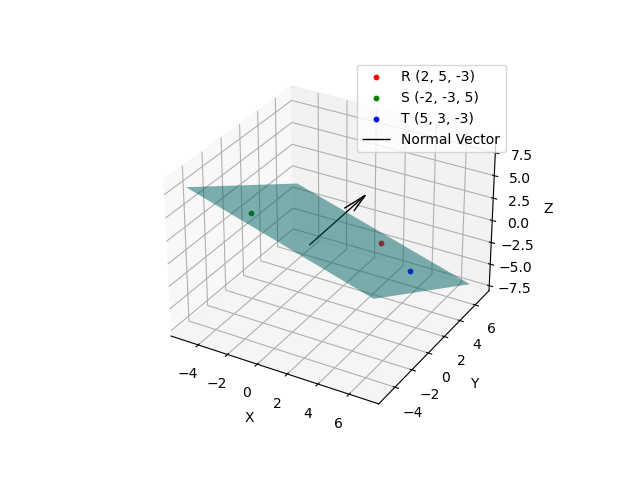
\includegraphics[width=0.6\linewidth]{figs/01.png}
   \caption{Plot of plane $\vec{n}^{T}\vec{x} = c$}
   \label{Plot_1}
\end{figure}
\end{document}
